\documentclass[17pt]{beamer} %Makes presentation
%\documentclass[handout, 17pt]{beamer} %Makes Handouts
\documentclass[14pt]{beamer} %Makes presentation
%\documentclass[handout]{beamer} %Makes Handouts
\usetheme{Singapore} %Gray with fade at top
\useoutertheme[subsection=false]{miniframes} %Supppress subsection in header
\useinnertheme{rectangles} %Itemize/Enumerate boxes
\usecolortheme{seagull} %Color theme
\usecolortheme{rose} %Inner color theme

\definecolor{light-gray}{gray}{0.75}
\definecolor{dark-gray}{gray}{0.55}
\setbeamercolor{item}{fg=light-gray}
\setbeamercolor{enumerate item}{fg=dark-gray}

\setbeamertemplate{navigation symbols}{}
%\setbeamertemplate{mini frames}[default]
\setbeamercovered{dynamics}
\setbeamerfont*{title}{size=\Large,series=\bfseries}

%\setbeameroption{notes on second screen} %Dual-Screen Notes
%\setbeameroption{show only notes} %Notes Output

\setbeamertemplate{frametitle}{\vspace{.5em}\bfseries\insertframetitle}
\newcommand{\heading}[1]{\noindent \textbf{#1}\\ \vspace{1em}}

\usepackage{bbding,color,multirow,times,ccaption,tabularx,graphicx,verbatim,booktabs,fixltx2e}
\usepackage{colortbl} %Table overlays
\usepackage[english]{babel}
\usepackage[latin1]{inputenc}
\usepackage[T1]{fontenc}
\usepackage{lmodern}

%\author[]{Thomas J. Leeper}
\institute[]{
  \inst{}%
  Department of Government\\London School of Economics and Political Science
}

\usepackage{tikz}
\usetikzlibrary{shapes,arrows,decorations.pathreplacing,calc}

\title{From Description\\ to Causation}

\date[]{}

\begin{document}

\frame{\titlepage}

\frame{\tableofcontents}


\frame{
\LARGE\centering\vskip10pt\textbf{What makes something a \textit{cause}?}

\vspace{1em}

\normalsize{Write for 1 minute.}

}

\section{Correlation vs. Causation}
\frame{\tableofcontents[currentsection]}


\frame{
\frametitle{Correlation}
\centering
Correlation is the \textit{non-independence} of two variables for a set of observations
}

\frame{
\includegraphics[width=\textwidth]{images/correlation.png}
}

\frame{
\frametitle{Correlation}

\begin{itemize}\itemsep1em
\item Synonyms: correlation, covariation, relationship, association
\item Any correlation is potentially causal
	\begin{itemize}
	\item X might cause Y
	\item Y might cause X
	\item X and Y might be caused by Z
	\item X and Y might cause Z
	\item There may be no causal relationship
	\end{itemize}
\end{itemize}
}



\frame{
\frametitle{Flashback!}

Two Categories of Inference:\\

\vspace{1em}

\begin{enumerate}\itemsep1em
\item Descriptive Inference
	\begin{itemize}
	\item What are the facts?
	\end{itemize}

\item Causal Inference
	\begin{itemize}
	\item Why does something occur?
	\end{itemize}
\end{enumerate}
}


\frame{

\frametitle{Correlation is Causation?}

\large\centering

The mind tends to interpret correlations and patterns as evidence of causal relationships!

\vspace{1em}

But this is rarely correct!

}


% gun violence and gun laws
\frame{
\centering
\includegraphics[height=.8\textheight]{images/gun_deaths.png}

\vspace{1em}

{\footnotesize Source: \href{https://commons.wikimedia.org/wiki/File:Gun_deaths_over_time_in_the_US_and_Australia.png}{Wikimedia Commons}}
}


% health care spending in countries
\frame{
\centering
\includegraphics[height=.8\textheight]{images/life_expectancy.png}

\vspace{1em}

{\footnotesize Source: \href{https://commons.wikimedia.org/wiki/File:Life_expectancy_vs_healthcare_spending.jpg}{Wikimedia Commons}}
}


% ecological correlations in voting patterns
\frame{
\centering
\includegraphics[width=\textwidth]{images/leave_vote_1.png}

\vspace{1em}

{\footnotesize Source: \href{https://www.economist.com/news/britain/21701950-areas-lots-migrants-voted-mainly-remain-or-did-they-britains-immigration-paradox}{\textit{The Economist}, 8 July 2016}}
}

\frame{
\centering
\includegraphics[width=\textwidth]{images/leave_vote_2.png}

\vspace{1em}

{\footnotesize Source: \href{https://www.economist.com/news/britain/21701950-areas-lots-migrants-voted-mainly-remain-or-did-they-britains-immigration-paradox}{\textit{The Economist}, 8 July 2016}}
}


% relationship between test scores in university admissions
\frame{
\centering
\includegraphics[height=.8\textheight]{images/quant-by-college-major-gender.png}

\vspace{1em}

{\footnotesize Source: \href{http://www.randalolson.com/2014/06/25/average-iq-of-students-by-college-major-and-gender-ratio/}{Randal Olson}}
}


% race and crime
\frame{
\centering
\includegraphics[width=\textwidth]{images/uk_race_crime.png}

\vspace{1em}

{\footnotesize Source: \href{https://www.gov.uk/government/uploads/system/uploads/attachment_data/file/219967/stats-race-cjs-2010.pdf}{Ministry of Justice, ``Statistics on Race and the Criminal Justice System 2010''}\par}
}




% chocolate and nobel prizes
\frame{
\centering
\includegraphics[height=.8\textheight]{images/chocolate_nobels.png}

\vspace{1em}

{\footnotesize Source: \href{https://stats.stackexchange.com/questions/36/examples-for-teaching-correlation-does-not-mean-causation}{StackExchange}}
}


% people drowning in pools and nicholas cage movies
\frame{
\centering
\includegraphics[width=\textwidth]{images/nicholascage.png}

{\footnotesize Source: \href{http://www.tylervigen.com/spurious-correlations}{TylerVigen.com}}
}



\frame{

\frametitle{Naive Causal Inference}

\begin{itemize}\itemsep1em
\item Correlations are not necessarily causal
\item Our mind thinks they are because humans are not very good at the kind of causal inference problems that social scientists care about
\item Instead, we're good at understanding \textit{physical} causality
\end{itemize}

}


\frame{
\frametitle{Physical causality}

\begin{itemize}\itemsep1em
\item Action and reaction
\item<2-> Example:
	\begin{itemize}
	\item Picture a ball resting on top of a hill
	\item What happens if I push the ball?
	\end{itemize}
\item<3-> Features:
	\begin{itemize}
	\item Observable
	\item Single-case
	\item Deterministic
	\item Monocausal
	\end{itemize}
\end{itemize}
}



\section{Over-Time Changes}
\frame{\tableofcontents[currentsection]}


\frame{

\frametitle{Pre-Post Change Heuristic}

\begin{itemize}\itemsep1em
\item Our intuition about causation relies too heavily on simple comparisons of \textit{pre-post change} in outcomes before and after something happens

	\begin{itemize}
	\item No change: no causation
	\item Increase in outcome: positive effect
	\item Decrease in outcome: negative effect
	\end{itemize}

\item<2-> Why is this flawed?
% monocausal
% could be alternative explanations for change or non-change
% in essence: pre-event outcomes are not necessarily a great counterfactual for post-event outcomes absent treatment
\end{itemize}

}

\frame{
\frametitle{Threats to Validity}

\centering
Campbell and Ross talk about six ``threats to validity'' (i.e., threats to causal inference) related to time-series analysis

}



\frame[label=threats]{

\frametitle{Flaws in causal inference from pre-post comparisons}

\begin{enumerate}
\item Maturation or trends
\item Regression to the mean
\item Selection
\item Simultaneous historical changes
\item Instrumentation changes
\item Monitoring changes behaviour
\end{enumerate}

}


\frame{
\frametitle{Maturation or trends}

\begin{itemize}\itemsep1em
\item Is a shift in an outcome before and after a policy change the impact of the policy or a small part of a longer time trend?

\item Case Study: Connecticut crackdown on speeding (1955)
\end{itemize}

}

\frame{
\centering
\includegraphics[height=\textheight]{images/campbell-1.png}
}


\frame{
\frametitle{Regression to the mean}

\begin{itemize}\itemsep1em
\item Is a shift in an outcome before and after a policy change the impact of the policy or a function of statistical variation?

\item Case Study: Connecticut crackdown on speeding (1955)
\end{itemize}

}

\frame{
\centering
\includegraphics[height=\textheight]{images/campbell-2.png}
}

\frame{
\frametitle{Selection}

\begin{itemize}\itemsep1em
\item Is a shift in an outcome before and after a policy the impact of the policy or the result of the policy being implemented when outcomes are extreme?

\item Case Study: Connecticut crackdown on speeding (1955)
\end{itemize}

}

\frame{
\centering
\includegraphics[height=\textheight]{images/campbell-2.png}
}

\frame{
\frametitle{Simultaneous changes}

\begin{itemize}\itemsep1em
\item Is the shift in an outcome before and after a policy the impact of the policy or the result of a simultaneous historical shift?

\item Case Study: US Great Depression Policy
\end{itemize}
}

\frame{
\includegraphics[width=\textwidth]{images/great-depression-gdp.png}
}


\frame{
\frametitle{Instrumentation changes}

\begin{itemize}\itemsep1em
\item Is the shift in an outcome before and after a policy the impact of the policy or a change in how the outcome is measured?

\item Case Study: Age-adjusted mortality rates
\end{itemize}

% http://www.rbtaylor.net/age_adjusted_rates.pdf
}

\frame{
\vspace{1em}
\includegraphics[width=\textwidth]{images/texas-cancer-rates.png}
}




\frame{
\frametitle{Monitoring changes behaviour}

\begin{itemize}\itemsep1em
\item Is the shift in an outcome before and after a policy the impact of the policy or a change in response to measuring the outcome per se?

\item Case Study: Educational testing
\end{itemize}
}

\frame{

\begin{quote}
The more any quantitative social indicator is used for social decision-making, the more subject it will be to corruption pressures and the more apt it will be to distort and corrupt the social processes it is intended to monitor.
\end{quote}

\raggedleft -- Donald T. Campbell (1979)

%achievement tests may well be valuable indicators of general school achievement under conditions of normal teaching aimed at general competence. But when test scores become the goal of the teaching process, they both lose their value as indicators of educational status and distort the educational process in undesirable ways.


}

\againframe{threats}

\frame{}

\frame{
	\includegraphics[width=\textwidth]{images/xkcdcorrelation.png}
}


\section{Getting Systematic about Causality}
\frame{\tableofcontents[currentsection]}


\frame{

\frametitle{{\large Directed Acyclic Graphs}}

\small

\begin{itemize}\itemsep0.5em
\item Causal graphs (DAGs) provide a visual representation of (possible) causal relationships
\item<2-> Causality flows between variables, which are represented as ``nodes''
	\begin{itemize}
	\item Variables are causally linked by arrows
	\item Causality only flows \textit{forward} in time
	\end{itemize}
\item<3-> Nodes opening a ``backdoor path'' from $X \rightarrow Y$ are confounds
	\begin{itemize}
	\item ``Selection bias'' or ``Confounding''
	\end{itemize}
\end{itemize}

}


\begin{frame}[label=smoking-graph]
\begin{center}
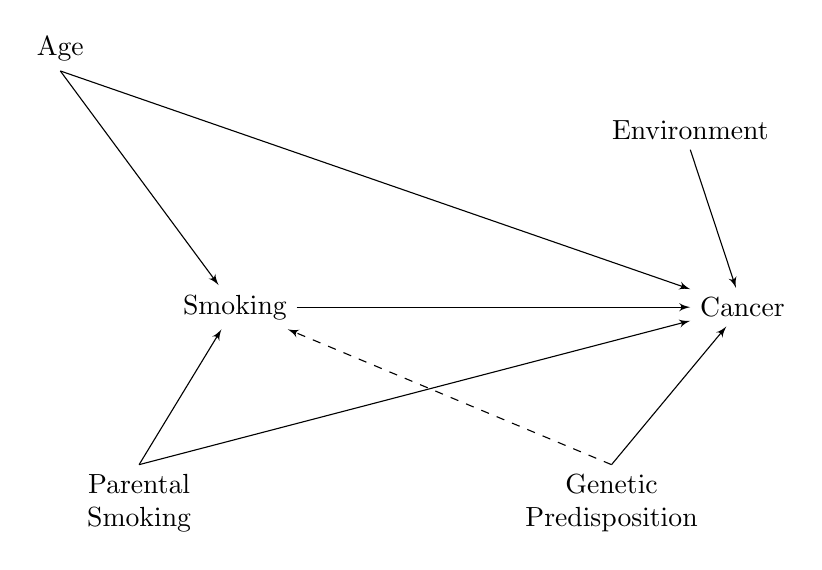
\begin{tikzpicture}[>=latex',circ/.style={draw, shape=circle, node distance=5cm, line width=1.5pt}]
    \draw (0,0) node[left] (X) {Smoking};
    \draw[->] (X) -- (5,0) node[right] (Y) {Cancer};
    \draw<2->[->] (-3,3) node[above] (Z) {Age} -- (Y);
    \draw<2->[->] (5,2) node[above] (A) {Environment} -- (Y);
    \draw<2->[->] (4,-2) node[below, text width=3cm, align=center] (E) {Genetic\\Predisposition} -- (Y);
    \draw<2->[->] (-2, -2) node[below, text width=2.5cm, align=center] (W) {Parental\\Smoking} -- (Y);
    \draw<3->[->] (Z.south) -- (X);
    \draw<3->[->] (W.north) -- (X);
    \draw<4->[->, dashed] (E.north) -- (X);
    %\draw<4->[<->, dashed] (W.west) -- (X.west);
\end{tikzpicture}
\end{center}
\end{frame}

\frame{

\frametitle{Causal Inference}

\centering

Causal inference (typically) involves gathering data in a systematic fashion in order to assess the size and form of correlation between nodes $X$ and $Y$ in such a way that there are no backdoor paths between $X$ and $Y$ by \textit{controlling for} (i.e., \textit{conditioning on}, \textit{holding constant}) any confounding variables, $\mathbf{Z}$.

}


\appendix
\frame{}

\end{document}
